\chapter{Fondamenti Teorici}
\label{chap:fondamenti_teorici}

La simulazione accurata del volo spaziale a vela solare richiede una modellazione rigorosa dell'ambiente fisico in cui il veicolo opera. Prima di procedere con l'implementazione degli algoritmi informatici all'interno del motore grafico, è indispensabile definire il \textit{background} matematico che descrive i limiti dei propulsori tradizionali, le leggi della meccanica orbitale e i modelli vettoriali che intervengono nella spinta fotonica. L'obiettivo di questo capitolo è fornire tutte le conoscenze che costituiranno il nucleo del simulatore numerico in Unreal Engine.

%%%%%%%%%%%%%%%%%%%%%%%%%%%%%%%%%%%%%%%%%%%%%%%%%%%%%%%%%%%%%%%%%%%%%%%%%%%%%%%%%%%%%%%%%%%%%%%%%%%%%
%%%%%%%%%%%%%%%%%%%%%%%%%%%%%%%%%%%%%%%%%%%%%%%%%%%%%%%%%%%%%%%%%%%%%%%%%%%%%%%%%%%%%%%%%%%%%%%%%%%%%

\section{I limiti fisici e termodinamici della propulsione chimica}
Per comprendere la necessità ingegneristica di sviluppare tecnologie a vela solare per lo spazio profondo, è opportuno analizzare matematicamente i problemi della propulsione spaziale tradizionale. Il limite insuperabile dei razzi chimici risiede nella dipendenza diretta tra la massa del propellente trasportato e la variazione di velocità ottenibile dal veicolo, un problema che la meccanica classica modella con estrema rigidità.

%%%%%%%%%%%%%%%%%%%%%%%%%%%%%%%%%%%%%%%%%%%%%%%%%%%%%%%%%%%%%%%%%%%%%%%%%%%%%%%%%%%%%%%%%%%%%%%%%%%%%

\subsection{Conservazione della quantità di moto ed equazione del razzo}
Il principio di funzionamento di un qualsiasi propulsore chimico si basa sulla terza legge della dinamica di Newton e sul principio di conservazione della quantità di moto. In un sistema chiuso, in assenza di forze esterne, la variazione totale della quantità di moto deve essere nulla.

Considerando un veicolo spaziale che espelle massa (propellente) a una velocità di scarico $v_e$, la quantità di moto totale del sistema (veicolo + propellente) deve rimanere costante. Se $m$ è la massa del veicolo in un dato istante e $dv$ è la variazione infinitesimale della sua velocità, mentre $dm$ è la variazione infinitesimale della massa (negativa, poiché il propellente viene espulso), si può scrivere:

\begin{equation}
    m \cdot dv = -v_e \cdot dm
\end{equation}

Riorganizzando i termini per separare le variabili, si ottiene l'equazione differenziale fondamentale del moto a propulsione chimica:

\begin{equation}
    dv = -v_e \frac{dm}{m}
\end{equation}

Integrando questa equazione tra lo stato iniziale (velocità $v_0$ e massa $m_0$) e lo stato finale (velocità $v_f$ e massa $m_f$), supponendo che la velocità di espulsione dei gas $v_e$ rimanga costante per tutta l'accensione, si ottiene:

\begin{equation}
    \int_{v_0}^{v_f} dv = -v_e \int_{m_0}^{m_f} \frac{1}{m} dm
\end{equation}

Il risultato di questa integrazione è la celebre equazione del razzo di Tsiolkovsky, formulata alla fine del XIX secolo dal fisico russo Konstantin Tsiolkovsky, che quantifica la variazione di velocità totale $\Delta v$ ottenibile dal razzo in funzione della massa iniziale, finale e della velocità di scarico:

\begin{equation} \label{eq:tsiolkovsky}
    \Delta v = v_e \ln\left(\frac{m_0}{m_f}\right) = I_{sp} \cdot g_0 \cdot \ln\left(\frac{m_0}{m_f}\right)
\end{equation}

dove i parametri fondamentali sono così definiti:
\begin{itemize}
    \item $v_e$ è la velocità effettiva di scarico dei gas.
    \item $I_{sp} = v_e / g_0$ è l'impulso specifico del propulsore, misurato in secondi, che rappresenta l'efficienza con cui la massa propellente viene convertita in spinta.
    \item $g_0$ è l'accelerazione di gravità standard al livello del mare ($9.80665 \, \text{m/s}^2$).
    \item $m_0$ è la massa iniziale al lancio, data dalla somma della massa a vuoto (struttura e \textit{payload}) e dalla massa del propellente.
    \item $m_f$ è la massa finale, ovvero la sola massa a vuoto una volta esaurito il propellente.
\end{itemize}

%%%%%%%%%%%%%%%%%%%%%%%%%%%%%%%%%%%%%%%%%%%%%%%%%%%%%%%%%%%%%%%%%%%%%%%%%%%%%%%%%%%%%%%%%%%%%%%%%%%%%

\subsection{Il rapporto di massa e la "tirannia" dell'equazione}
L'equazione \ref{eq:tsiolkovsky} mette in luce un problema fondamentale per l'ingegneria aerospaziale. Invertendo la formula per isolare il rapporto di massa (definito come $\Lambda = m_0/m_f$), si ottiene:

\begin{equation}
    \Lambda = \frac{m_0}{m_f} = e^{\frac{\Delta v}{I_{sp} \cdot g_0}}
\end{equation}

Questa relazione esponenziale è spesso definita come "tirannia dell'equazione del razzo". Essa dimostra che la massa iniziale richiesta cresce in modo esponenziale rispetto alla variazione di velocità desiderata \cite{mcinnes1999solar}. 

Attraverso un esempio pratico è possibile chiarire questo concetto.
Se si desidera raddoppiare il $\Delta v$ di una missione mantenendo costante il carico utile e il tipo di motore, non è sufficiente raddoppiare il propellente. Sarà necessario trasportare una quantità di carburante esponenzialmente maggiore, poiché il propulsore dovrà spendere energia per accelerare anche il carburante stesso che non è stato ancora espulso. Per le missioni interplanetarie dirette verso destinazioni distanti dal sistema solare, i requisiti di $\Delta v$ rendono il rapporto $\Lambda$ talmente elevato da lasciare una frazione di massa per il carico scientifico (\textit{payload}) inferiore all'1\% / 2\% della massa totale al momento del lancio \cite{johnson2012status}.

\begin{figure}[htbp!]
    \centering
    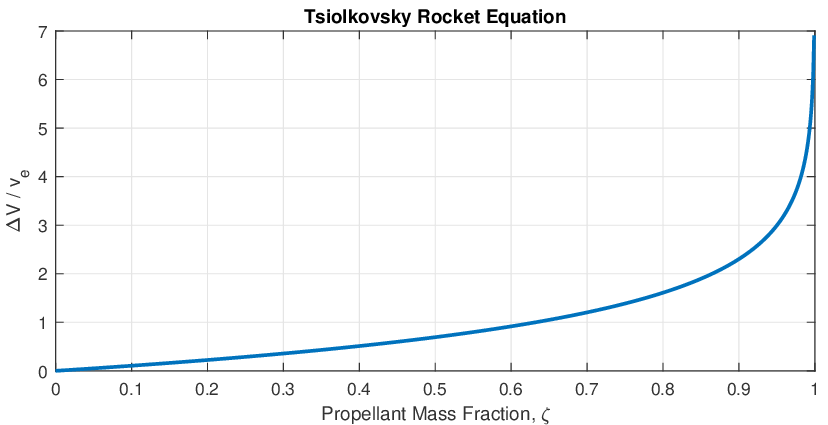
\includegraphics[width=0.7\textwidth]{Images/tsiolkovsky_graph.png}
    \caption{Rappresentazione grafica della "tirannia dell'equazione del razzo": la massa iniziale necessaria cresce in modo esponenziale all'aumentare della variazione di velocità richiesta ($\Delta v$).}
    \label{fig:tsiolkovsky_graph}
\end{figure}

%%%%%%%%%%%%%%%%%%%%%%%%%%%%%%%%%%%%%%%%%%%%%%%%%%%%%%%%%%%%%%%%%%%%%%%%%%%%%%%%%%%%%%%%%%%%%%%%%%%%%

\subsection{Il vincolo termodinamico insuperabile}
Di fronte alla crescita esponenziale della massa, l'unica soluzione matematica per ridurre il carico di propellente è aumentare l'impulso specifico $I_{sp}$, o la velocità di scarico $v_e$. Tuttavia, nei motori chimici questo parametro non può essere aumentato arbitrariamente. 

La velocità di espulsione dei gas è strettamente vincolata dal calore massimo che la reazione chimica riesce a sprigionare e dalla leggerezza dei prodotti che generano la spinta. Pur ricorrendo alla miscela propulsiva più efficiente a disposizione dell'ingegneria aerospaziale (idrogeno e ossigeno allo stato liquido, LOX/LH2), il limite termodinamico teorico dell'impulso specifico si scontra con una soglia invalicabile di circa 450-460 secondi. Semplicemente, nessuna reazione chimica conosciuta possiede un'intensità energetica sufficiente per superare questa barriera naturale.

Con dei limiti prestazionali così severi, l'esplorazione umana nello spazio profondo incontra una barriera fisica invalicabile \cite{mcconnell2023solarcruiser}. È in questo panorama di difficoltà termodinamiche che si inserisce la necessità di sviluppare propulsori di natura non-chimica. 
Se un veicolo potesse attingere la propria quantità di moto dall'esterno, eliminando del tutto la massa di propellente ($m_0 \approx m_f$), l'equazione di Tsiolkovsky decadrebbe, offrendo un impulso specifico potenzialmente infinito. Questa è l'esatta premessa teorica su cui si fonda la propulsione a vela solare.

%%%%%%%%%%%%%%%%%%%%%%%%%%%%%%%%%%%%%%%%%%%%%%%%%%%%%%%%%%%%%%%%%%%%%%%%%%%%%%%%%%%%%%%%%%%%%%%%%%%%%
%%%%%%%%%%%%%%%%%%%%%%%%%%%%%%%%%%%%%%%%%%%%%%%%%%%%%%%%%%%%%%%%%%%%%%%%%%%%%%%%%%%%%%%%%%%%%%%%%%%%%

\section{Fisica della radiazione elettromagnetica e pressione solare}
L'esplorazione sostenibile dello spazio profondo, quindi, richiede un cambio di strategia propulsiva che svincoli il veicolo dall'equazione di Tsiolkovsky. La propulsione a vela solare risponde a questa esigenza attingendo a una fonte di energia esterna e inesauribile: il Sole. Tuttavia, per comprendere matematicamente in che modo un raggio di luce possa generare una spinta meccanica tangibile su un oggetto macroscopico, è necessario esplorare la natura quantistica della radiazione elettromagnetica e definire le grandezze fisiche che governano l'ambiente interplanetario.

%%%%%%%%%%%%%%%%%%%%%%%%%%%%%%%%%%%%%%%%%%%%%%%%%%%%%%%%%%%%%%%%%%%%%%%%%%%%%%%%%%%%%%%%%%%%%%%%%%%%%

\subsection{Il dualismo onda-particella e la quantità di moto del fotone}
Dal punto di vista della fisica classica, la luce è descritta dalle equazioni dell'elettromagnetismo formulate da James Clerk Maxwell nel 1873. Secondo questo modello, la radiazione solare è un'onda elettromagnetica che si propaga nello spazio e che, incidendo su una superficie, esercita una pressione derivante dalla forza di Lorentz applicata alle cariche elettriche del materiale investito.

Sebbene il modello ondulatorio confermi l'esistenza della pressione di radiazione, la sua classificazione moderna si appoggia in modo più completo alla meccanica quantistica, in particolar modo riguardo alla propulsione. Nel 1905, Albert Einstein, spiegando l'effetto fotoelettrico, teorizzò che la luce non fosse unicamente un'onda continua, ma fosse quantizzata in pacchetti di energia, successivamente chiamati "fotoni".

Questa scoperta diede origine al concetto di \textit{dualismo onda-particella}, successivamente formalizzato e analizzato da Louis de Broglie. Un fotone è una particella elementare priva di massa ($m_0 = 0$). Tuttavia, secondo l'equazione dell'energia relativistica di Einstein:

\begin{equation}
    E^2 = (pc)^2 + (m_0 c^2)^2
\end{equation}

\begin{itemize}
    \item $E$ è l'energia totale della particella
    \item $p$ è la quantità di moto
    \item $c$ è la velocità della luce nel vuoto ($299\,792\,458 \, \text{m/s}$)
\end{itemize}

Ponendo la massa a riposo $m_0$ pari a zero, l'equazione si riduce a un'uguaglianza fondamentale per l'astrodinamica delle vele solari:

\begin{equation} \label{eq:quantita_moto_fotone}
    E = p \cdot c \implies p = \frac{E}{c}
\end{equation}

Questa relazione quantistica elementare è il cuore della propulsione fotonica \cite{mcinnes1999solar}. Essa dimostra che ogni singolo fotone che colpisce la membrana di una vela solare trasporta una quantità di moto infinitesimale. Quando il fotone viene assorbito o riflesso dalla superficie, la sua quantità di moto subisce una variazione ($\Delta p$). Per il principio di conservazione della quantità di moto, questa variazione deve essere trasferita alla vela sotto forma di impulso meccanico, generando una forza continua nel tempo.

%%%%%%%%%%%%%%%%%%%%%%%%%%%%%%%%%%%%%%%%%%%%%%%%%%%%%%%%%%%%%%%%%%%%%%%%%%%%%%%%%%%%%%%%%%%%%%%%%%%%%

\subsection{Costante solare e pressione in orbita terrestre}
Un singolo fotone possiede un'energia estremamente piccola. Affinché il trasferimento di quantità di moto diventi sufficiente per muovere un veicolo spaziale di svariati chilogrammi, è necessario calcolare l'effetto del flusso luminoso emesso da una stella.

Il Sole irradia energia in tutte le direzioni e la quantità di energia solare che attraversa perpendicolarmente una superficie unitaria in un secondo è definita come \textit{irradianza}. Alla distanza media tra la Terra e il Sole, definita come Unità Astronomica ($1 \, \text{AU} \approx 149.6 \times 10^6 \, \text{km}$), questo flusso prende il nome di \textbf{Costante Solare} ($W_E$). 

I dati moderni stabiliscono che il valore medio della costante solare all'esterno dell'atmosfera terrestre è:

\begin{equation}
    W_E \approx 1361 \, \text{W/m}^2 \quad \left( \text{oppure } \frac{\text{J}}{\text{s} \cdot \text{m}^2} \right)
\end{equation}

Sfruttando la relazione di Einstein ricavata in precedenza (Equazione \ref{eq:quantita_moto_fotone}), è possibile convertire questo flusso di energia in una pressione meccanica. Dividendo l'irradianza per la velocità della luce, si ottiene la pressione nominale della radiazione solare ($P_E$) misurata a un'Unità Astronomica di distanza su una superficie teorica perfettamente assorbente:

\begin{equation} \label{eq:pressione_terrestre}
    P_E = \frac{W_E}{c} = \frac{1361}{299\,792\,458} \approx 4.56 \times 10^{-6} \, \text{N/m}^2
\end{equation}

Questo valore estremamente piccolo (pari a circa 4.56 micronewton per metro quadrato) evidenzia il primo problema della propulsione a vela solare: la forza generata da un singolo metro quadrato di membrana è infinitesimale. Per ottenere una spinta significativa, è necessario dispiegare vele di dimensioni enormi (centinaia o migliaia di metri quadrati) e operare in un ambiente privo di attriti aerodinamici, come lo spazio interplanetario \cite{rodrigues2023review}.

%%%%%%%%%%%%%%%%%%%%%%%%%%%%%%%%%%%%%%%%%%%%%%%%%%%%%%%%%%%%%%%%%%%%%%%%%%%%%%%%%%%%%%%%%%%%%%%%%%%%%

\subsection{Decadimento spaziale e legge dell'inverso del quadrato}
La costante $P_E$ calcolata è valida esclusivamente nelle vicinanze dell'orbita terrestre (orbite LEO, MEO, GEO). Tuttavia, un simulatore astrodinamico progettato per missioni interplanetarie deve modellare dinamicamente la variazione della spinta in funzione della posizione del veicolo nel sistema solare.

L'energia emessa dal Sole si propaga radialmente e, poiché l'area di una sfera cresce proporzionalmente al quadrato del suo raggio ($A = 4\pi r^2$), la densità dei fotoni (e di conseguenza la pressione di radiazione) subisce una diminuzione quadratica.

Definendo $r_E$ come la distanza di riferimento (1 AU) e $r$ come l'effettiva distanza tra il Sole e la vela solare nell'istante di tempo considerato, l'intensità della pressione locale $P(r)$ è governata dalla legge dell'inverso del quadrato:

\begin{figure}[htbp!]
    \centering
    \includegraphics[width=0.75\textwidth]{Images/inverse_square_law.jpg}
    \caption{Propagazione sferica della radiazione elettromagnetica: la densità dei fotoni e la relativa pressione diminuiscono con il quadrato della distanza dalla sorgente solare.}
    \label{fig:inverse_square_law}
\end{figure}

\begin{equation} \label{eq:pressione_locale}
    P(r) = P_E \left( \frac{r_E}{r} \right)^2
\end{equation}

Questa equazione impone un vincolo molto preciso, che grazie al simulatore software sarà possibile verificare in tempo reale: la spinta di una vela solare non è costante, ma decresce rapidamente man mano che il veicolo si allontana dal Sole.
Avvicinandosi al Sole (ad esempio verso Venere o Mercurio, come avvenuto per la sonda IKAROS), il denominatore $r$ diminuisce, causando un incremento quadratico della spinta propulsiva e del carico termico. Al contrario, dirigendosi verso i pianeti esterni (Giove, Saturno), la pressione solare crolla drasticamente \cite{johnson2012status}. Ad esempio, a 5 AU (l'orbita di Giove), la spinta fotonica si riduce a solo 1/25 del valore misurato sulla Terra, rendendo le manovre a vela solare estremamente lente e complesse nello spazio profondo \cite{rodrigues2023review}.

%%%%%%%%%%%%%%%%%%%%%%%%%%%%%%%%%%%%%%%%%%%%%%%%%%%%%%%%%%%%%%%%%%%%%%%%%%%%%%%%%%%%%%%%%%%%%%%%%%%%%

\subsection{Luminosità solare}
Sebbene l'utilizzo della Costante Solare ($P_E$) sia comune per le missioni riferite unicamente all'orbita terrestre, lo sviluppo di un simulatore astrodinamico complesso richiede un approccio più generalizzato. 
Ecco perché un approccio più universale consiste nel calcolare la pressione di radiazione a partire dalla potenza totale emessa dal Sole, ovvero la sua luminosità ($L$), e adattare dinamicamente il calcolo in base alla posizione del veicolo.

Difatti il Sole si comporta come un'enorme lampada sferica che irradia energia in tutte le direzioni. La potenza totale emessa dal Sole è una costante fisica, espressa in $W$ che può essere calcolata a partire dalla Costante Solare e dall'area della sfera di raggio 1 AU:

\begin{equation}
    L \approx 3.828 \times 10^{26} \, \text{W}
\end{equation}

Poiché questa immensa energia si propaga nello spazio vuoto distribuendosi sulla superficie di una sfera in continua espansione (la cui area è $4\pi r^2$), il flusso energetico locale a una qualsiasi distanza $r$ dal centro del Sole è dato da:

\begin{equation}
    W(r) = \frac{L}{4 \pi r^2} \quad \left[ \frac{\text{W}}{\text{m}^2} \right]
\end{equation}

\begin{figure}[htbp!]
    \centering
    % 
\includegraphics[width=0.8\textwidth]{Images/inverse_square_luminosity.jpg}
    \caption{Rappresentazione geometrica della Legge dell'Inverso del Quadrato: la Potenza totale emessa dalla stella (Luminosità L) si diluisce sulla superficie di sfere concentriche in espansione, riducendo l'intensità del flusso locale in proporzione a $1/r^2$.}
    \label{fig:luminosity_inverse_square}
\end{figure}

Dividendo questo flusso per la velocità della luce $c$, si ottiene l'equazione universale della pressione fotonica locale con cui è possibile calcolare la forza istantanea che agisce su una vela solare in qualsiasi punto del sistema solare:

\begin{equation} \label{eq:pressione_luminosita}
    P(r) = \frac{L}{4 \pi r^2 c}
\end{equation}

Questa formulazione è più flessibile e adatta a un simulatore astrodinamico, poiché consente di modellare con precisione la spinta fotonica in qualsiasi punto del sistema solare, tenendo conto della posizione dinamica del veicolo rispetto al Sole. È proprio questa equazione che è stata implementata nel simulatore sviluppato in Unreal Engine, permettendo il calcolo istantaneo della pressione di radiazione locale e dell'accelerazione risultante durante l'intero arco della missione.

%%%%%%%%%%%%%%%%%%%%%%%%%%%%%%%%%%%%%%%%%%%%%%%%%%%%%%%%%%%%%%%%%%%%%%%%%%%%%%%%%%%%%%%%%%%%%%%%%%%%%
%%%%%%%%%%%%%%%%%%%%%%%%%%%%%%%%%%%%%%%%%%%%%%%%%%%%%%%%%%%%%%%%%%%%%%%%%%%%%%%%%%%%%%%%%%%%%%%%%%%%%

\section{Modellazione ottica vettoriale e interazione fotonica}
Avendo definito la pressione di radiazione solare locale $P(r)$, è possibile calcolare la forza totale che agisce su una vela solare. Tuttavia, questa forza non è semplicemente il prodotto scalare tra $P(r)$ e l'area geometrica della vela. La spinta risultante dipende da una complessa interazione tra i fotoni incidenti e la superficie della membrana, che coinvolge fenomeni di riflessione, assorbimento e diffusione.

%%%%%%%%%%%%%%%%%%%%%%%%%%%%%%%%%%%%%%%%%%%%%%%%%%%%%%%%%%%%%%%%%%%%%%%%%%%%%%%%%%%%%%%%%%%%%%%%%%%%%

\subsection{Area effettiva e angolo di incidenza}
Il primo parametro fondamentale per calcolare l'interazione fotonica è la determinazione della parte della vela effettivamente esposta al flusso di fotoni. La forza generata dalla pressione solare non dipende dall'area totale della vela, ma dall'area proiettata perpendicolarmente alla direzione dei raggi solari.

Per prima cosa è necessario definire un sistema di riferimento solidale alla vela solare in cui $\mathbf{n}$ rappresenta il versore normale (perpendicolare) alla superficie della vela. Inoltre, è utile dichiarare $\mathbf{u}$ come il versore direzione dell'illuminazione, ovvero il vettore che punta dal centro di massa del veicolo verso il Sole. 

L'angolo compreso tra il versore normale $\mathbf{n}$ e la direzione dei raggi solari $\mathbf{u}$ prende il nome di \textit{angolo di incidenza} ($\alpha$). 
La superficie della vela non sempre è completamente esposta al flusso solare. L'area effettiva che riceve i fotoni dipende dall'orientamento della vela rispetto al Sole ed è calcolata così:

\begin{equation}
    A_{\text{eff}} = A \cos(\alpha)
\end{equation}

\begin{figure}[htbp!]
    \centering
    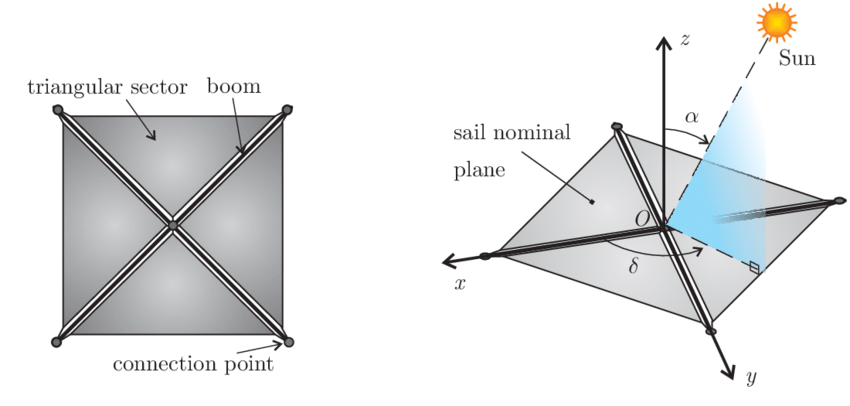
\includegraphics[width=0.6\textwidth]{Images/sail_geometry.png}
    \caption{Schema vettoriale dell'interazione fotonica: il versore normale $\mathbf{n}$, la direzione dei raggi solari $\mathbf{u}$ e l'angolo di incidenza $\alpha$ che determina l'area effettivamente esposta.}
    \label{fig:sail_geometry}
\end{figure}

Questa relazione geometrica implica che la vela cattura il massimo della quantità di moto quando è orientata frontalmente al Sole ($\alpha = 0^\circ$, dove $\cos(0) = 1$). Man mano che la vela viene inclinata, l'area esposta diminuisce, fino ad annullarsi completamente quando la vela è posta "di taglio" rispetto ai raggi solari ($\alpha = 90^\circ$, dove $\cos(90) = 0$).

%%%%%%%%%%%%%%%%%%%%%%%%%%%%%%%%%%%%%%%%%%%%%%%%%%%%%%%%%%%%%%%%%%%%%%%%%%%%%%%%%%%%%%%%%%%%%%%%%%%%%

\subsection{Fenomeni di ombreggiamento e auto-occlusione}
Il modello matematico finora descritto assume che la vela solare sia una superficie piana e perfettamente esposta ai raggi solari. Nella realtà operativa, tuttavia, la sonda è una struttura tridimensionale complessa. Elementi come il modulo centrale (\textit{bus}), i bracci telescopici per il dispiegamento (\textit{booms}) e la strumentazione di bordo sono posti tra il Sole e la vela riflettente, proiettando delle ombre.

Questo fenomeno, noto come \textbf{auto-occlusione}, azzera la spinta fotonica nelle zone oscurate. Le conseguenze sulla dinamica del veicolo sono due: 
\begin{itemize}
    \item Una riduzione netta della spinta propulsiva totale.
    \item Uno spostamento asimmetrico del centro di pressione; questo può generare un momento torcente che induce rotazioni non pianificate del veicolo, complicando le manovre di controllo d'assetto.
\end{itemize}

Oltre a ciò, la vela può presentare deformazioni strutturali, pieghe o irregolarità che causano ulteriori ombre.

Per calcolare con precisione l'area effettivamente illuminata, l'equazione algebrica $A_{\text{eff}} = A \cos(\alpha)$ non basta.
Il calcolo deve essere impostato come un integrale di superficie che includa una funzione di visibilità $v(x,y)$, la quale restituisce il valore $1$ se il punto è direttamente illuminato e il valore $0$ se è in ombra:

\begin{equation}
    A_{\text{eff}} = \int_{A} v(x,y) \cos(\alpha) \, dA
\end{equation}

\begin{figure}[htbp!]
    \centering
    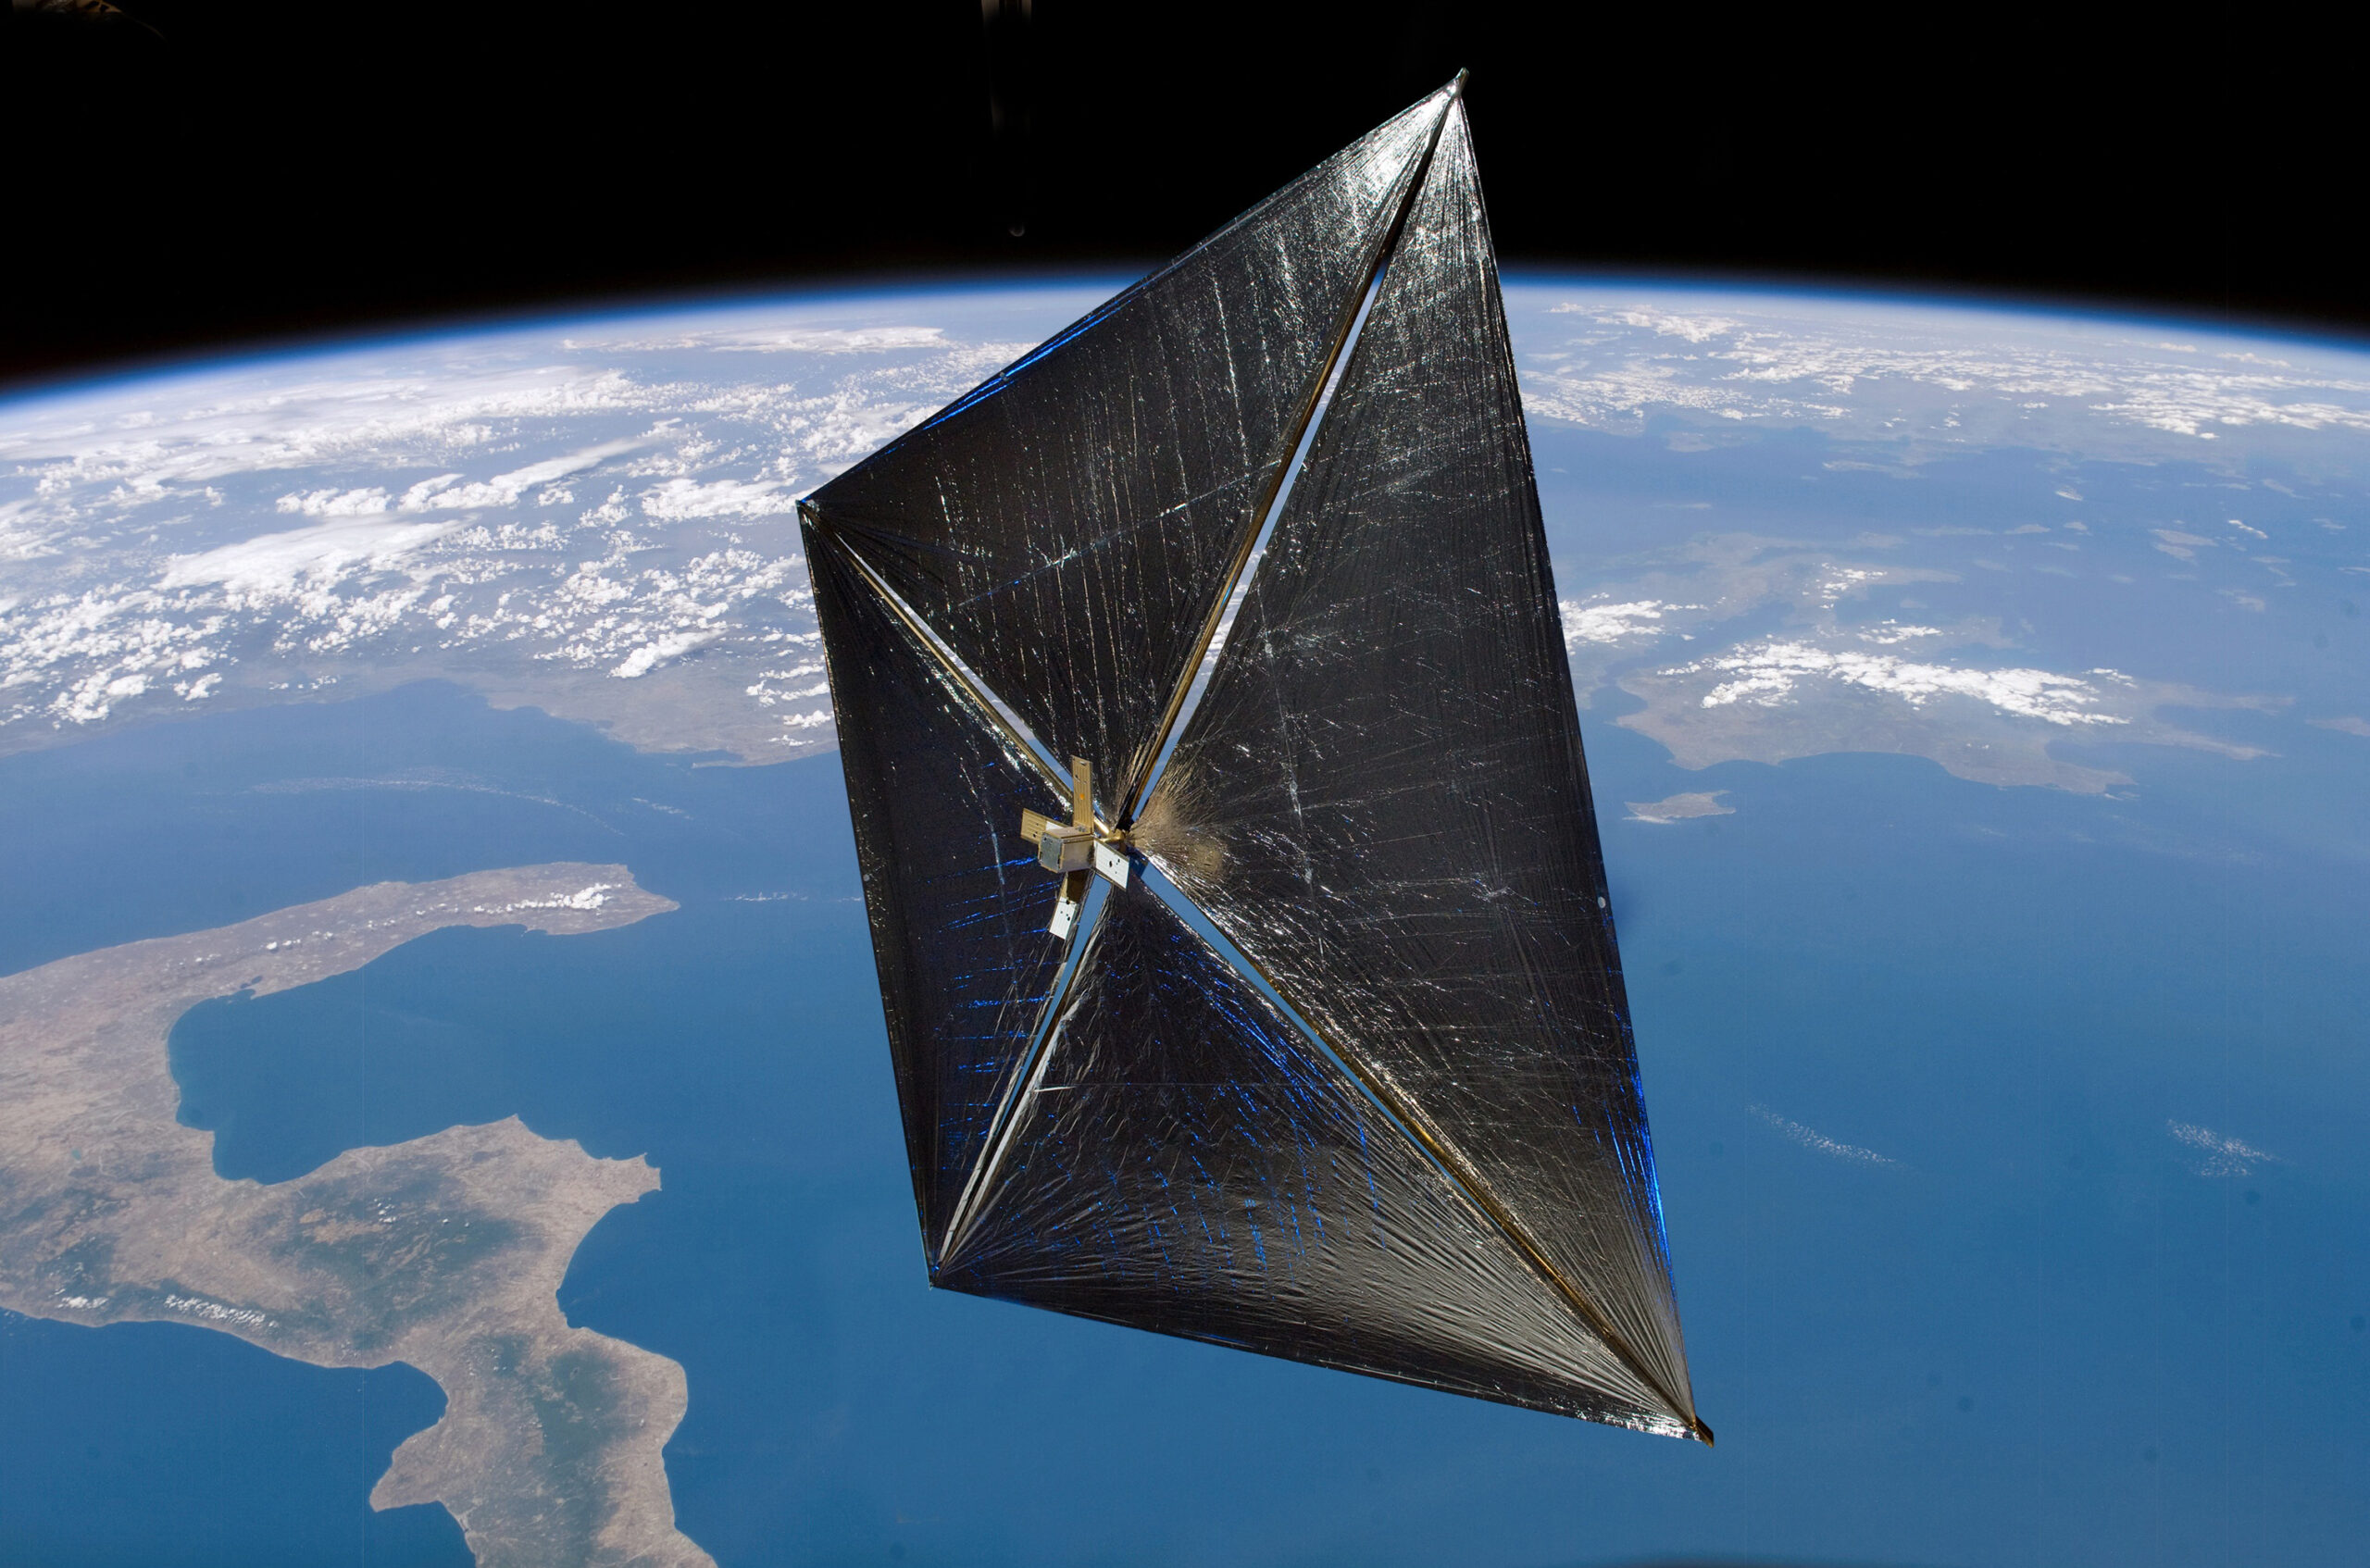
\includegraphics[width=0.7\textwidth]{Images/sail_shadowing.jpg}
    \caption{Rappresentazione concettuale dell'auto-occlusione: i componenti strutturali del veicolo proiettano ombre sulla membrana riflessiva, rendendo necessario il calcolo locale dell'area effettivamente illuminata.}
    \label{fig:sail_shadowing}
\end{figure}

Purtroppo questo calcolo risulta essere impossibile da risolvere analiticamente, poiché la funzione di visibilità $v(x,y)$ dipende dalla geometria complessa del veicolo e dalla posizione relativa del Sole.
Questo ostacolo giustifica la necessità di utilizzare un motore grafico: algoritmi di calcolo spaziale discretizzato, come il \textit{Ray Casting}, permettono di campionare dinamicamente la funzione di visibilità $v(x,y)$ sulla geometria della vela, risolvendo il problema delle ombre in tempo reale.

%%%%%%%%%%%%%%%%%%%%%%%%%%%%%%%%%%%%%%%%%%%%%%%%%%%%%%%%%%%%%%%%%%%%%%%%%%%%%%%%%%%%%%%%%%%%%%%%%%%%%

\subsection{Occlusione ambientale e asimmetria di spinta}
Oltre all'auto-occlusione causata dai componenti specifici della vela solare, un simulatore astrodinamico ad alta fedeltà deve modellare accuratamente l'\textbf{occlusione ambientale}. Questo fenomeno si verifica quando un corpo celeste (ad esempio un pianeta, una luna o un asteroide) si interpone tra il Sole e la vela, causando un'occlusione totale o parziale.

Se un'eclissi totale comporta semplicemente l'azzeramento globale della spinta fotonica, le fasi di transizione o di occlusione parziale introducono problemi molto più complessi. Quando un corpo oscura solo una porzione della vela solare, si instaura una forte asimmetria nella distribuzione delle forze. 

Dal punto di vista della meccanica dei corpi rigidi, la differenza di pressione causata dalla radiazione solare, tra la zona in ombra e la superficie illuminata, dà luogo ad una discordanza tra i due centri di pressione fotonica e di massa del veicolo, generando un momento torcente che provoca la rotazione del veicolo.

Il simulatore sviluppato in questo elaborato è capace di analizzare questa complessa casistica.
In particolar modo, grazie alla modellazione tridimensionale della vela solare e alla simulazione dinamica del sistema solare, è possibile calcolare in tempo reale l'effetto di un'eclissi parziale, prevedendo con precisione la forza risultante e il momento torcente che agisce sul veicolo durante le fasi di transizione.


\begin{figure}[htbp!]
    \centering
    % 
\includegraphics[width=0.7\textwidth]{Images/partial_eclipse_torque.jpg}
    \caption{Effetto dell'occlusione ambientale parziale: l'asimmetria di illuminazione sposta il centro di pressione rispetto al centro di massa, generando un momento torcente (\textit{torque}) che induce il rotolamento del veicolo.}
    \label{fig:eclipse_torque}
\end{figure}

L'effetto di questo momento torcente è di fondamentale importanza per la dinamica del veicolo, poiché può indurre un "rotolamento" incontrollato che a sua volta può compromettere l'orientamento dei pannelli solari e interrompere i collegamenti telemetrici con la Terra. Inoltre costringe il sistema di controllo d'assetto a consumare preziose risorse propulsive per contrastare queste rotazioni, riducendo ulteriormente l'efficienza complessiva della missione \cite{rodrigues2023review}.

%%%%%%%%%%%%%%%%%%%%%%%%%%%%%%%%%%%%%%%%%%%%%%%%%%%%%%%%%%%%%%%%%%%%%%%%%%%%%%%%%%%%%%%%%%%%%%%%%%%%%

\subsection{Il modello ottico ideale (Riflessione speculare perfetta)}
Per comprendere l'origine delle componenti di forza, è utile partire da un modello ideale in cui la superficie della vela solare è perfettamente liscia e riflettente, senza alcuna perdita di energia.
In questo scenario ideale, si assume che il 100\% dei fotoni incidenti venga riflesso in modo perfettamente elastico (riflessione speculare), senza alcuna perdita di energia per assorbimento o diffusione. 

Quando un fotone con quantità di moto $p$ colpisce la superficie con un angolo $\alpha$, esso viene riflesso con il medesimo angolo rispetto alla normale. La variazione della quantità di moto del fotone lungo l'asse tangenziale alla vela è nulla, mentre lungo l'asse normale alla vela è pari a $2p \cos(\alpha)$. 

Integrando questo scambio di quantità di moto sull'intera area esposta $A \cos(\alpha)$ e moltiplicandolo per il flusso di fotoni, si ottiene la forza della Pressione di Radiazione Solare nel caso ideale ($\mathbf{F}_{\text{ideale}}$). Poiché in un urto elastico la componente trasversale si annulla, l'intero vettore forza è diretto lungo la normale $\mathbf{n}$ della vela:

\begin{equation} \label{eq:srp_ideale}
    \mathbf{F}_{\text{ideale}} = 2 P(r) A \cos^2(\alpha) \mathbf{n}
\end{equation}
Per comprendere l'origine del termine $\cos^2(\alpha)$, è necessario analizzare in dettaglio l'interazione fotonica per ogni singolo fotone incidente.
Considerando un fotone incidente che trasporta quantità di moto $p = E/c$. 

Quando il fotone colpisce la superficie della vela con angolo di incidenza $\alpha$ (misurato rispetto alla normale $\mathbf{n}$), la sua quantità di moto può essere ripartita in due componenti perpendicolari tra loro:
\begin{itemize}
    \item Componente normale: $p_n = p \cos(\alpha)$
    \item Componente tangenziale: $p_t = p \sin(\alpha)$
\end{itemize}

Nel caso di riflessione speculare perfetta, il fotone rimbalza elasticamente mantenendo l'angolo di incidenza. La componente tangenziale rimane invariata ($p_t' = p_t$), mentre la componente normale si inverte ($p_n' = -p_n$). La variazione totale di quantità di moto del fotone lungo la direzione normale è:

\begin{equation}
    \Delta p_n = p_n' - p_n = -p\cos(\alpha) - p\cos(\alpha) = -2p\cos(\alpha)
\end{equation}

Per il principio di conservazione della quantità di moto, la vela riceve un impulso diretto lungo la propria normale pari a:

\begin{equation}
    \Delta p_{\text{vela}} = 2p\cos(\alpha) = 2\frac{E}{c}\cos(\alpha)
\end{equation}

Tuttavia, il flusso luminoso non interagisce con l'intera area geometrica $A$ della membrana, bensì soltanto con la porzione effettivamente esposta alla radiazione, la quale si riduce all'aumentare dell'inclinazione del veicolo:

\begin{equation}
    A_{\text{eff}} = A\cos(\alpha)
\end{equation}

La forza totale esercitata sulla vela si ricava integrando la pressione locale $P(r)$ sull'area effettiva, tenendo conto del fattore di riflessione elastica lungo la normale. Moltiplicando questi termini si ottiene:

\begin{equation}
    F = P(r) \cdot A_{\text{eff}} \cdot (2\cos\alpha) = 2P(r)A\cos^2(\alpha)
\end{equation}

Il termine quadratico $\cos^2(\alpha)$ è di fondamentale importanza nell'astrodinamica fotonica e ha una duplice origine fisica: un primo fattore $\cos(\alpha)$ deriva dalla riduzione puramente geometrica dell'area intercettata ($A_{\text{eff}}$), mentre il secondo $\cos(\alpha)$ deriva dalla proiezione dell'impulso trasferito lungo l'asse normale alla superficie.

Questa dipendenza quadratica dimostra che la spinta di una vela solare diminuisce molto rapidamente rispetto alla semplice inclinazione della vela: a $30^\circ$ di incidenza, la forza propulsiva si riduce al $75\%$ del suo valore ($\cos^2(30^\circ) \approx 0.75$), a $45^\circ$ di inclinazione invece la forza scende al $50\%$ \cite{mcinnes1999solar}.

%%%%%%%%%%%%%%%%%%%%%%%%%%%%%%%%%%%%%%%%%%%%%%%%%%%%%%%%%%%%%%%%%%%%%%%%%%%%%%%%%%%%%%%%%%%%%%%%%%%%%

\subsection{Il modello ottico realistico (Superfici non ideali)}
Il modello ideale descritto dall'Equazione \ref{eq:srp_ideale} è un'ottima approssimazione per i calcoli preliminari, ma risulta inadeguato per un simulatore informatico \textit{High-Fidelity}. Nella realtà, nessun materiale polimerico metallizzato (come il Kapton alluminato) possiede una riflettività del 100\%. 

L'interazione della luce con un materiale reale è un fenomeno complesso in cui i fotoni incidenti subiscono rimbalzi differenti. Per modellare matematicamente questo comportamento, la letteratura aerospaziale definisce tre coefficienti ottici, la cui somma conserva l'energia totale (deve essere pari a 1):

\begin{equation}
    \rho_s + \rho_d + \alpha_a = 1
\end{equation}

Questi parametri descrivono le tre reazioni ottiche della superficie:
\begin{itemize}
    \item \textbf{Riflessione speculare ($\rho_s$):} La parte di fotoni che rimbalza elasticamente mantenendo l'angolo di incidenza. Genera una forza diretta unicamente lungo la normale $\mathbf{n}$.
    \item \textbf{Riflessione diffusa ($\rho_d$):} La parte di fotoni che, a causa delle irregolarità del materiale, viene riflessa in direzioni casuali. Questa componente introduce una forza di taglio parallela alla superficie della vela, deviando la forza totale rispetto alla normale $\mathbf{n}$.
    \item \textbf{Assorbimento ($\alpha_a$):} La frazione di fotoni che non viene riflessa, ma assorbita dal materiale. Questa componente non genera "rimbalzo", trasferendo la propria quantità di moto esclusivamente nella direzione di incidenza originale dei raggi solari ($\mathbf{u}$). L'energia assorbita si trasforma poi in calore termico.
\end{itemize}

\begin{figure}[htbp!]
    \centering
    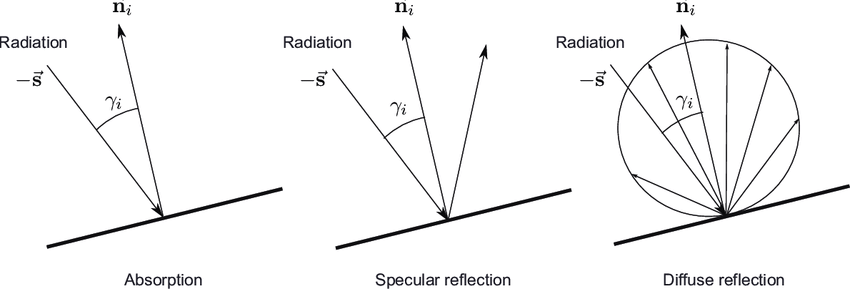
\includegraphics[width=0.8\textwidth]{Images/optical_reflection_model.png}
    \caption{Confronto visivo tra i fenomeni ottici su una superficie non ideale: riflessione speculare ($\rho_s$), riflessione diffusa ($\rho_d$) e assorbimento ($\alpha_a$).}
    \label{fig:optical_model}
\end{figure}

La coesistenza di questi tre fenomeni fa sì che la forza risultante su una vela reale non sia mai perfettamente allineata al versore normale $\mathbf{n}$ (tranne quando $\alpha = 0^\circ$). L'assorbimento e la diffusione introducono un'asimmetria che genera una forza di taglio (\textit{shear force}) parallela alla superficie della vela, un elemento critico che può deviare la traiettoria orbitale.

%%%%%%%%%%%%%%%%%%%%%%%%%%%%%%%%%%%%%%%%%%%%%%%%%%%%%%%%%%%%%%%%%%%%%%%%%%%%%%%%%%%%%%%%%%%%%%%%%%%%%

\subsection{L'equazione vettoriale dell'accelerazione SRP}
Volendo quindi determinare l'effettiva spinta generata sul veicolo, i valori derivanti dai diversi fenomeni ottici descritti devono essere raggruppati in un'unica formula. Per la buona riuscita di questa operazione, si introduce il versore trasversale $\mathbf{t}$, definito come parallelo al piano della vela solare e complanare al piano formato dalla normale $\mathbf{n}$ e dalla direzione di incidenza dei raggi solari $\mathbf{u}$.

L'accelerazione totale generata dalla Pressione di Radiazione Solare ($\mathbf{a}_{\text{SRP}}$) su un veicolo di massa $m$ e area $A$, inclinato di un angolo $\alpha$ lungo la direzione del versore $\mathbf{t}$, è espressa dalla seguente equazione vettoriale \cite{simo2016realistic}:

\begin{equation} \label{eq:srp_force_vector}
    \mathbf{a}_{\text{SRP}} = \frac{P(r) A}{m} \cos(\alpha) \left[ \left(1 + \rho_s \cos(2\alpha) + \frac{2}{3}\rho_d \cos(\alpha) \right)\mathbf{n} + \left(\rho_s \sin(2\alpha) + \rho_d \sin(\alpha) \right)\mathbf{t} \right]
\end{equation}

Questa formulazione mostra l'intera fisica propulsiva del modello non-ideale. Al suo interno è possibile distinguere chiaramente due valori ortogonali: 
\begin{itemize}
    \item La componente associata al versore $\mathbf{n}$ rappresenta la \textbf{spinta normale}, ovvero l'accelerazione generata lungo la direzione normale alla superficie della vela.
    \item La componente associata al versore $\mathbf{t}$ rappresenta la \textbf{forza di taglio} (\textit{shear force}), elemento critico per la navigazione solare poiché in grado di generare spostamenti laterali della traiettoria orbitale.
\end{itemize}

Calcolare questa espressione vettoriale istante per istante, ricavando ogni volta le normali geometriche $\mathbf{n}$ e osservando come i raggi incidono sulla vela, rappresenta la prima sfida che il simulatore software in C++, sviluppata in Unreal Engine e presentata nel capitolo successivo, deve svolgere.

%%%%%%%%%%%%%%%%%%%%%%%%%%%%%%%%%%%%%%%%%%%%%%%%%%%%%%%%%%%%%%%%%%%%%%%%%%%%%%%%%%%%%%%%%%%%%%%%%%%%%
%%%%%%%%%%%%%%%%%%%%%%%%%%%%%%%%%%%%%%%%%%%%%%%%%%%%%%%%%%%%%%%%%%%%%%%%%%%%%%%%%%%%%%%%%%%%%%%%%%%%%

\section{Parametri di design e sintesi della dinamica orbitale}
Attraverso le equazioni esposte nei paragrafi precedenti, è possibile calcolare con precisione la forza di pressione solare che agisce su una vela in qualsiasi punto del sistema solare, tenendo conto dell'orientamento della vela e delle proprietà ottiche del materiale.
Tuttavia, il reale comportamento cinematico del veicolo spaziale sottoposto alla perturbazione solare non dipende esclusivamente dall'efficienza ottica del materiale o dalla distanza dal Sole, ma è rigidamente vincolata dalla geometria strutturale e dalla distribuzione delle masse del veicolo. Ecco perché diventa utile definire alcuni parametri di design che sintetizzano le caratteristiche macroscopiche del veicolo e che permettono di valutare le prestazioni propulsive in modo più immediato, indipendentemente dall'orbita specifica o dalle condizioni operative.

%%%%%%%%%%%%%%%%%%%%%%%%%%%%%%%%%%%%%%%%%%%%%%%%%%%%%%%%%%%%%%%%%%%%%%%%%%%%%%%%%%%%%%%%%%%%%%%%%%%%%

\subsection{Il Carico Alare (Sail Loading)}
Il parametro di design più critico nella progettazione di un veicolo a propulsione fotonica è il Carico Alare (\textit{Sail Loading}), solitamente indicato con la lettera greca $\sigma$. Questo è definito come il rapporto tra la massa totale del veicolo spaziale e l'area totale della membrana dispiegata per la "cattura" dei fotoni:

\begin{equation} \label{eq:sail_loading}
    \sigma = \frac{m}{A} \quad \left[ \frac{\text{kg}}{\text{m}^2} \right]
\end{equation}

La massa $m$ al numeratore comprende tutti i componenti del veicolo: la massa del carico utile (\textit{payload} scientifico), la massa riguardante i sistemi satellitari (sistemi di comunicazione, computer di bordo, pannelli solari, giroscopi per la rotazione della vela), la massa dei bracci telescopici di dispiegamento (\textit{booms}) e, infine, la massa della membrana stessa.

L'obiettivo primario durante il dimensionamento di una missione è minimizzare $\sigma$. Un valore di \textit{Sail Loading} basso indica infatti che il veicolo è molto leggero rispetto alla superficie che espone alla radiazione solare, massimizzando così l'accelerazione generata dalla pressione di radiazione.
Le vele solari di prima generazione (come IKAROS) presentavano valori di $\sigma$ relativamente alti a causa dell'utilizzo di membrane più spesse e meccanismi di dispiegamento delle stesse più pesanti. Attraverso gli sviluppi moderni e futuri si può mirare a spingere questo valore al di sotto dei $10 \, \text{g/m}^2$, impiegando pellicole di spessore sub-micrometrico e strutture in fibra di carbonio, che sono in grado di resistere alle sollecitazioni meccaniche e termiche dello spazio profondo pur mantenendo una massa estremamente ridotta \cite{rodrigues2023review} \cite{johnson2012status}.

%%%%%%%%%%%%%%%%%%%%%%%%%%%%%%%%%%%%%%%%%%%%%%%%%%%%%%%%%%%%%%%%%%%%%%%%%%%%%%%%%%%%%%%%%%%%%%%%%%%%%

\subsection{Accelerazione Caratteristica}
Un altro parametro di design fondamentale è l'Accelerazione Caratteristica ($a_c$). Esso rappresenta il valore massimo di accelerazione che una vela solare può generare quando è esposta alla luce solare nelle condizioni più favorevoli: posizionata a 1 Unità Astronomica dal Sole e orientata perpendicolarmente rispetto ai raggi solari ($\alpha = 0^\circ$).

Sostituendo l'equazione del \textit{Sail Loading} ($\sigma$) all'interno del modello ottico realistico discusso in precedenza (Equazione \ref{eq:srp_force_vector}), e considerando che per $\alpha = 0^\circ$ la componente trasversale si annulla, si ricava la formula analitica dell'Accelerazione Caratteristica:

\begin{equation} \label{eq:accelerazione_caratteristica}
    a_c = \frac{P_E}{\sigma} \left( 1 + \rho_s + \frac{2}{3}\rho_d \right) \quad \left[ \frac{\text{m}}{\text{s}^2} \right]
\end{equation}

Questo valore rappresenta un fondamentale parametro di riferimento per la validazione dell'ambiente virtuale. Al fine di certificare l'accuratezza del simulatore, durante le fasi di collaudo i vettori tridimensionali restituiti in tempo reale da Unreal Engine dovranno essere confrontati con il valore $a_c$ teorico, a patto che la vela simulata venga esposta alle condizioni operative ideali.

%%%%%%%%%%%%%%%%%%%%%%%%%%%%%%%%%%%%%%%%%%%%%%%%%%%%%%%%%%%%%%%%%%%%%%%%%%%%%%%%%%%%%%%%%%%%%%%%%%%%%

\subsection{Numero di Leggerezza}
Un ulteriore parametro di design di grande interesse astrodinamico è il Numero di Leggerezza (\textit{Lightness Number}, $\beta$). Esso esprime il rapporto tra la massima accelerazione repulsiva della pressione solare $a_c$ e l'attrazione gravitazionale del Sole $g_{\text{sole}}$ alla stessa distanza:

\begin{equation}
    \beta = \frac{a_c}{g_{\text{sole}}}
\end{equation}

Il Numero di Leggerezza è un valore che mostra rapidamente la capacità propulsiva di una vela solare rispetto alla forza gravitazionale che agisce su di essa. Un valore di $\beta < 1$ indica che la forza gravitazionale del Sole vince su quella fotonica, di conseguenza la vela non potrà mai "sfuggire" dal sistema solare e per acquisire velocità dovrà rimanere in orbita per molto. Al contrario, un valore di $\beta > 1$ indica che la spinta fotonica supera la gravità solare, permettendo al veicolo di "sfuggire" direttamente dal sistema solare seguendo una traiettoria iperbolica, senza necessità di lunghi periodi di accelerazione orbitale \cite{mcinnes1999solar}.

%%%%%%%%%%%%%%%%%%%%%%%%%%%%%%%%%%%%%%%%%%%%%%%%%%%%%%%%%%%%%%%%%%%%%%%%%%%%%%%%%%%%%%%%%%%%%%%%%%%%%

\subsection{Il campo gravitazionale primario e la meccanica orbitale}
Seppur fino ad ora si sia parlato esclusivamente delle forze riguardanti la dinamica fotonica, è importante evidenziare che la vela solare è comunque sempre soggetta alla forza gravitazionale di uno o più corpi celesti.

Il veicolo fotonico è infatti governato dalle leggi della meccanica orbitale, ed in particolar modo dalla legge di gravitazione universale formulata da Isaac Newton.
Questa afferma che ogni corpo dotato di massa esercita un'attrazione gravitazionale su ogni altro corpo, con una forza $\mathbf{F}_g$ che è direttamente proporzionale al prodotto delle loro masse e inversamente proporzionale al quadrato della distanza che unisce i due centri di massa:

\begin{equation}
    \mathbf{F}_g = - G \frac{M \cdot m}{r^2} \mathbf{\hat{r}}
\end{equation}

dove:
\begin{itemize}
    \item $G$ è la Costante di Gravitazione Universale ($6.674 \times 10^{-11} \, \text{m}^3 \text{kg}^{-1} \text{s}^{-2}$), fondamentale che quantifica l'intensità gravitazionale;
    \item $M$ è la massa del corpo centrale, espressa in $\text{kg}$, che genera il campo gravitazionale;
    \item $m$ è la massa del veicolo spaziale, che subisce l'attrazione gravitazionale generata dal corpo centrale;
    \item $r$ è la distanza tra i centri di massa del corpo centrale e del veicolo spaziale, misurata in metri;
    \item $\mathbf{\hat{r}}$ è il versore che indica la direzione dal centro del pianeta verso il veicolo spaziale, con il segno negativo che indica che la forza è attrattiva (verso il corpo centrale).
\end{itemize}


Affinché il veicolo spaziale non venga attratto verso il corpo centrale, è necessario che la forza di gravità sia controbilanciata da una forza centrifuga generata dal moto orbitale del veicolo.
Questa velocità orbitale, che dipende dalla distanza $r$ e dalla massa del corpo centrale $M$, è quella necessaria per mantenere un'orbita stabile.

Tale velocità si ricava uguagliando la forza gravitazionale alla forza centrifuga ($m v^2 / r$) e risolvendo per $v$, ottenendo così la formula della velocità orbitale circolare:

\begin{equation}
    v = \sqrt{\frac{G \cdot M}{r}}
\end{equation}

La moltiplicazione tra $G$ e $M$ è un prodotto così ricorrente nella meccanica orbitale che viene spesso accorpato in un unico parametro, noto come \textit{parametro gravitazionale standard} ($\mu$) definito come:

\begin{equation}
    \mu = G \cdot M
\end{equation}

È dunque possibile esprimere anche la forza gravitazionale in termini di accelerazione, dividendo $\mathbf{F}_g$ per la massa del veicolo $m$:

\begin{equation}
    \mathbf{a}_g = \frac{\mathbf{F}_g}{m} = - G \frac{M}{r^2} \mathbf{\hat{r}} = - \frac{\mu}{r^2} \mathbf{\hat{r}}
\end{equation}
 
Inoltre, tenendo conto che il versore $\mathbf{\hat{r}}$ è definito come $\mathbf{r}/r$, dove $\mathbf{r}$ è il vettore posizione del veicolo spaziale rispetto al corpo centrale è possibile esprimere tale accelerazione in forma vettoriale.
Infine quindi, l'equazione vettoriale dell'accelerazione gravitazionale centrale che agisce su un veicolo spaziale in orbita attorno a un corpo centrale è:

\begin{equation}
    \mathbf{a}_g(\mathbf{r}) = - \frac{\mu}{r^3} \mathbf{r}
\end{equation}

\begin{figure}[htbp!]
    \centering
    % \includegraphics[width=0.6\textwidth]{Images/gravity_vector_diagram.jpg}
    \caption{Diagramma vettoriale dell'accelerazione gravitazionale centrale. Il vettore posizione $\mathbf{r}$ è diretto dal fuoco all'oggetto; il vettore accelerazione $\mathbf{a}_g$ è sempre diretto in verso opposto (verso il corpo attrattore), giustificando il segno negativo nell'equazione vettoriale.}
    \label{fig:gravity_vector}
\end{figure}

%%%%%%%%%%%%%%%%%%%%%%%%%%%%%%%%%%%%%%%%%%%%%%%%%%%%%%%%%%%%%%%%%%%%%%%%%%%%%%%%%%%%%%%%%%%%%%%%%%%%%

\subsection{Sintesi finale: l'Equazione del Moto}
Ora che sono state definite sia gravità ($\mathbf{a}_g$) che spinta fotonica ($\mathbf{a}_{\text{SRP}}$), è possibile unirle per ottenere l'equazione finale che descrive il movimento della vela solare.

Per mantenere il calcolo gestibile, si ricorre solitamente a un'approssimazione pratica: vengono ignorate le forze secondarie marginali, come l'attrito dell'alta atmosfera, l'attrazione della Luna o la forma non perfettamente sferica della Terra. Fatto ciò, l'accelerazione totale della navicella è semplicemente la somma di chi la tira verso il basso (il pianeta) e di chi la spinge via (il Sole):

\begin{equation} \label{eq:equazione_moto_finale}
    \ddot{\mathbf{r}} = \mathbf{a}_g(\mathbf{r}) + \mathbf{a}_{\text{SRP}}(\mathbf{r}, \alpha, \rho_s, \rho_d)
\end{equation}

Espandendo questa formula e inserendo tutte le equazioni che sono state dimostrate fino ad ora, compreso l'uso della Luminosità solare ($L$) per calcolare la pressione, è possibile ottenere l'equazione completa del sistema:

\begin{equation}
    \frac{d^2\mathbf{r}}{dt^2} = - \frac{\mu}{r^3} \mathbf{r} + \frac{L \cdot A}{4 \pi r^2 c \cdot m} \cos(\alpha) \left[ \left(1 + \rho_s \cos(2\alpha) + \frac{2}{3}\rho_d \cos(\alpha) \right)\mathbf{n} + \left(\rho_s \sin(2\alpha) + \rho_d \sin(\alpha) \right)\mathbf{t} \right]
\end{equation}

\begin{figure}[htbp!]
    \centering
    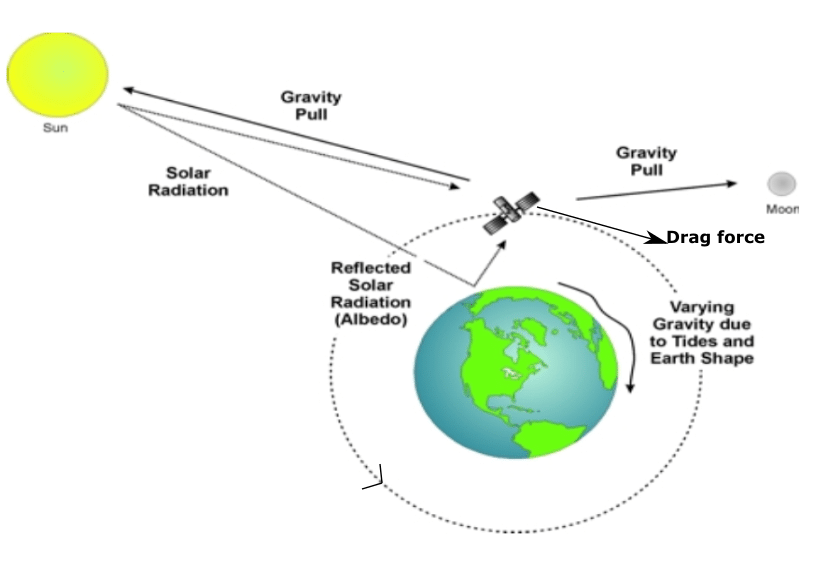
\includegraphics[width=0.7\textwidth]{Images/orbital_forces.png}
    \caption{Diagramma delle forze in gioco: l'accelerazione totale della vela solare è data dalla somma vettoriale tra la gravità ($\mathbf{a}_g$) e la perturbazione fotonica ($\mathbf{a}_{\text{SRP}}$).}
    \label{fig:orbital_forces}
\end{figure}

Come è facile intuire, questa equazione è estremamente complessa. Tale complessità rende notevolmente difficile la possibilità di prevedere con precisione la traiettoria del veicolo spaziale, poiché ogni variabile è in continua evoluzione durante il viaggio. Man mano che il veicolo viaggia, la distanza ($r$) varia, modificando contemporaneamente sia l'attrazione gravitazionale che l'intensità della luce. Inoltre, ogni minima rotazione della vela cambia gli angoli di incidenza e i vettori di direzione ($\mathbf{n}$ e $\mathbf{t}$).

A causa di queste continue variazioni, è matematicamente impossibile risolvere questa equazione "a mano" con carta e penna per prevedere dove si troverà la vela tra un mese. L'unico modo per tracciare la rotta è usare un approccio virtuale: far calcolare al computer questa enorme formula ogni istante. Il prossimo capitolo spiegherà proprio come la programmazione a oggetti e il motore grafico Unreal Engine 5 siano stati impiegati per compiere questo complesso lavoro.

%%%%%%%%%%%%%%%%%%%%%%%%%%%%%%%%%%%%%%%%%%%%%%%%%%%%%%%%%%%%%%%%%%%%%%%%%%%%%%%%%%%%%%%%%%%%%%%%%%%%%
%%%%%%%%%%%%%%%%%%%%%%%%%%%%%%%%%%%%%%%%%%%%%%%%%%%%%%%%%%%%%%%%%%%%%%%%%%%%%%%%%%%%%%%%%%%%%%%%%%%%%